\section{Moments and Centroids}


Consider a mass-less rod that is balanced on a fulcrum. If we place a block with mass $m$ a distance of $2l$ to the right of the fulcrum, intuitively, the rod will rotate clockwise. If we want to balance the rod, laws of Physics tell us that we can place two blocks on the left side, a distance $l$ from the fulcrum.

\vspace{0.5cm}

\begin{center}
\resizebox{3in}{!}{
\tikzset{every picture/.style={line width=0.75pt}}
\begin{tikzpicture}[x=0.75pt,y=0.75pt,yscale=-1,xscale=1]
%uncomment if require: \path (0,300); %set diagram left start at 0, and has height of 300

%Shape: Triangle [id:dp41533082302553526]
\draw   (313.8,191.4) -- (348.6,299.33) -- (278.6,299.33) -- cycle ;
%Shape: Rectangle [id:dp7864068096012333]
\draw   (45,182.33) -- (584.5,182.33) -- (584.5,190) -- (45,190) -- cycle ;
%Shape: Rectangle [id:dp44305625383026936]
\draw   (549,113.33) -- (619,113.33) -- (619,182) -- (549,182) -- cycle ;
%Shape: Rectangle [id:dp8062085686265645]
\draw   (155,113.33) -- (225,113.33) -- (225,182) -- (155,182) -- cycle ;
%Shape: Rectangle [id:dp4577443473497005]
\draw   (155,44.67) -- (225,44.67) -- (225,113.33) -- (155,113.33) -- cycle ;
%Shape: Brace [id:dp7912317035658136]
\draw   (191,190) .. controls (190.99,194.67) and (193.31,197.01) .. (197.98,197.02) -- (242.23,197.14) .. controls (248.9,197.16) and (252.22,199.5) .. (252.21,204.17) .. controls (252.22,199.5) and (255.56,197.18) .. (262.23,197.2)(259.23,197.19) -- (306.48,197.32) .. controls (311.15,197.33) and (313.49,195.01) .. (313.5,190.34) ;
%Shape: Brace [id:dp037948391723723995]
\draw   (314.2,190.6) .. controls (314.21,195.27) and (316.54,197.6) .. (321.21,197.59) -- (439.36,197.47) .. controls (446.03,197.46) and (449.36,199.79) .. (449.36,204.46) .. controls (449.36,199.79) and (452.69,197.46) .. (459.36,197.45)(456.36,197.45) -- (577.51,197.32) .. controls (582.18,197.32) and (584.51,194.99) .. (584.5,190.32) ;

% Text Node
\draw (254,219) node    {\huge$l$};
% Text Node
\draw (450,220) node   [align=left] {\huge$\displaystyle 2l$};
% Text Node
\draw (190,147.67) node    {\huge$m$};
% Text Node
\draw (190,79) node    {\huge$m$};
% Text Node
\draw (584,147.67) node    {\huge$m$};


\end{tikzpicture}}
\end{center}

% \vspace{0.5cm}

We need to find a way to quantify how much placing a weight on the rod makes the rod want to turn: let's borrow a concept from Physics and define the \textbf{moment} of the arrangement of masses. By convention, we will say that the moment is \textit{positive} if the arrangement suggests a clockwise rotation, \textit{negative} if the arrangement suggests a counterclockwise rotation, and \textit{zero} if the rod (sometimes called a moment arm) is balanced. Also, we will measure distances from the origin, (the \textbullet \ on the diagram below).

In order to model real physical phenomena, we define the moment:
$$
M=\sum_{i=1}^nx_im_i
$$
where $x_i$ is the signed distance from the origin of mass $m_i$.

For example, consider the following diagram.

\vspace{0.5cm}

\begin{center}
\resizebox{3in}{!}{
\tikzset{every picture/.style={line width=0.75pt}}
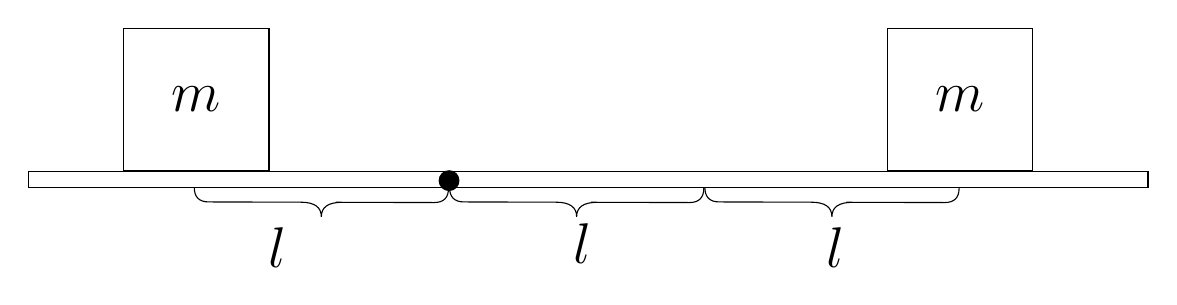
\begin{tikzpicture}[x=0.75pt,y=0.75pt,yscale=-1,xscale=1]
%uncomment if require: \path (0,300); %set diagram left start at 0, and has height of 300
%Shape: Rectangle [id:dp7864068096012333]
\draw   (62,176.33) -- (601.5,176.33) -- (601.5,184) -- (62,184) -- cycle ;
%Shape: Rectangle [id:dp44305625383026936]
\draw   (476,107.33) -- (546,107.33) -- (546,176) -- (476,176) -- cycle ;
%Shape: Rectangle [id:dp8062085686265645]
\draw   (108,107.33) -- (178,107.33) -- (178,176) -- (108,176) -- cycle ;
%Shape: Brace [id:dp7912317035658136]
\draw   (142,184) .. controls (141.99,188.67) and (144.31,191.01) .. (148.98,191.02) -- (193.23,191.14) .. controls (199.9,191.16) and (203.22,193.5) .. (203.21,198.17) .. controls (203.22,193.5) and (206.56,191.18) .. (213.23,191.2)(210.23,191.19) -- (257.48,191.32) .. controls (262.15,191.33) and (264.49,189.01) .. (264.5,184.34) ;
%Shape: Brace [id:dp5786950624316944]
\draw   (265,184) .. controls (264.99,188.67) and (267.31,191.01) .. (271.98,191.02) -- (316.23,191.14) .. controls (322.9,191.16) and (326.22,193.5) .. (326.21,198.17) .. controls (326.22,193.5) and (329.56,191.18) .. (336.23,191.2)(333.23,191.19) -- (380.48,191.32) .. controls (385.15,191.33) and (387.49,189.01) .. (387.5,184.34) ;
%Shape: Brace [id:dp4016151154645182]
\draw   (388,184) .. controls (387.99,188.67) and (390.31,191.01) .. (394.98,191.02) -- (439.23,191.14) .. controls (445.9,191.16) and (449.22,193.5) .. (449.21,198.17) .. controls (449.22,193.5) and (452.56,191.18) .. (459.23,191.2)(456.23,191.19) -- (503.48,191.32) .. controls (508.15,191.33) and (510.49,189.01) .. (510.5,184.34) ;
%Shape: Circle [id:dp29917281201395207]
\draw  [fill={rgb, 255:red, 0; green, 0; blue, 0 }  ,fill opacity=1 ] (260,180.75) .. controls (260,178.13) and (262.13,176) .. (264.75,176) .. controls (267.37,176) and (269.5,178.13) .. (269.5,180.75) .. controls (269.5,183.37) and (267.37,185.5) .. (264.75,185.5) .. controls (262.13,185.5) and (260,183.37) .. (260,180.75) -- cycle ;

% Text Node
\draw (182,213) node    {\huge$l$};
% Text Node
\draw (143,141.67) node    {\huge$m$};
% Text Node
\draw (511,141.67) node    {\huge$m$};
% Text Node
\draw (329,211) node    {\huge$l$};
% Text Node
\draw (451,213) node    {\huge$l$};


\end{tikzpicture}}
\end{center}

\vspace{0.5cm}

Here the moment is
$$M=\sum_{i=0}^2x_im_i=(2l)(m)+(-l)(m)=ml,$$
which is positive. This is as we hoped, since the arrangement of masses would intuitively rotate to the right around the origin.

If we have an arrangement of blocks with moment $M$ and total mass $A$, and we are interested in finding where to place the fulcrum to balance the rod, we want the \textbf{center of mass}, which is defined to be the location $\overline{x}$ that satisfies the equality:
$$
\overline{x}A=M.
$$

In other words, if we calculate the moment of the arrangement of masses that consists solely of the system mass $A$ at location $\overline{x}$, it would be equal to the moment of the original system. Another interpretation of the center of mass is the \underline{weighted} average location of all of the masses. That is, each mass has more influence on the average location if it is heavier. This is seen in the equation
$$\overline{x}=\frac{M}{A}=\frac{1}{A}\sum_{i=0}^nx_im_i.$$


Returning to our two-mass example, we can calculate
$$\overline{x}=\frac{(2l)(m)+(-l)(m)}{2m}=\frac{l}{2},$$
which should make sense since $\frac{l}{2}$ to the right of the origin is exactly between the two masses.

This method is interesting in a discrete system with finitely many masses, but we can use integrals to transition this same idea to continuous systems!

Suppose we are given two plotted functions $f$ and $g$ that enclose an area (mass distribution) $A$ in the plane, and we wish to find the center of mass along the $x$-axis.


\begin{center}
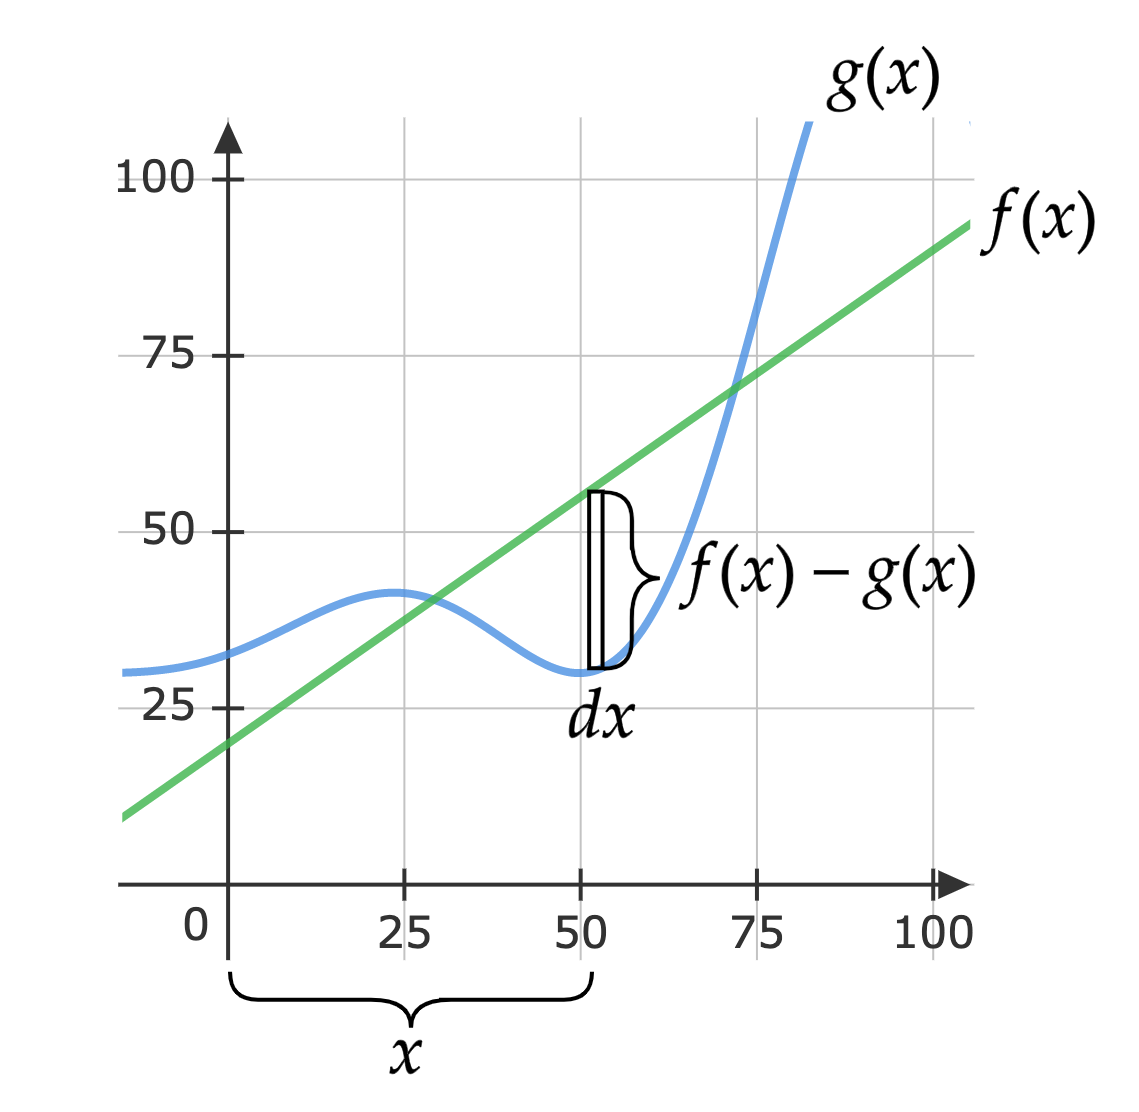
\includegraphics[width=3in]{img/moments_plot1.png}
\end{center}

As is illustrated in the figure, we can divide the mass area into infinitesimal slices between the endpoints $a$ and $b$, and sum them up. As before, each term is weighted with the signed distance along the moment arm ($x-axis$) to the origin $x$, and has the infinitesimal area (``mass'')
$$\underbrace{(f(x)-g(x))}_\text{height}\ \underbrace{dx}_\text{width}.$$
The following equation is the continuous analog of the equation for $\overline{x}$ above:
$$
\overline{x} = \frac{1}{A}\int_{x=a}^{x=b}x(f(x)-g(x))\ dx.
$$
If you are interested in finding $\overline{x}$ for the area under a function, then $g(x)=0$, so
$$
\overline{x} = \frac{1}{A}\int_{x=a}^{x=b}xf(x)\ dx.
$$
So far, we have only been considering a moment arm on the $x$-axis, but if we want to find the $y$ coordinate of the center of mass, we can use the same form, but instead of summing over slices along the $x$-axis, we integrate over the $y$-axis between end points $y=c$ and $y=d$:
$$
\overline{y} = \frac{1}{A}\int_{y=c}^{y=d}y(p(y)-q(y))\ dy.
$$
See the figure below for a visual:


\begin{center}
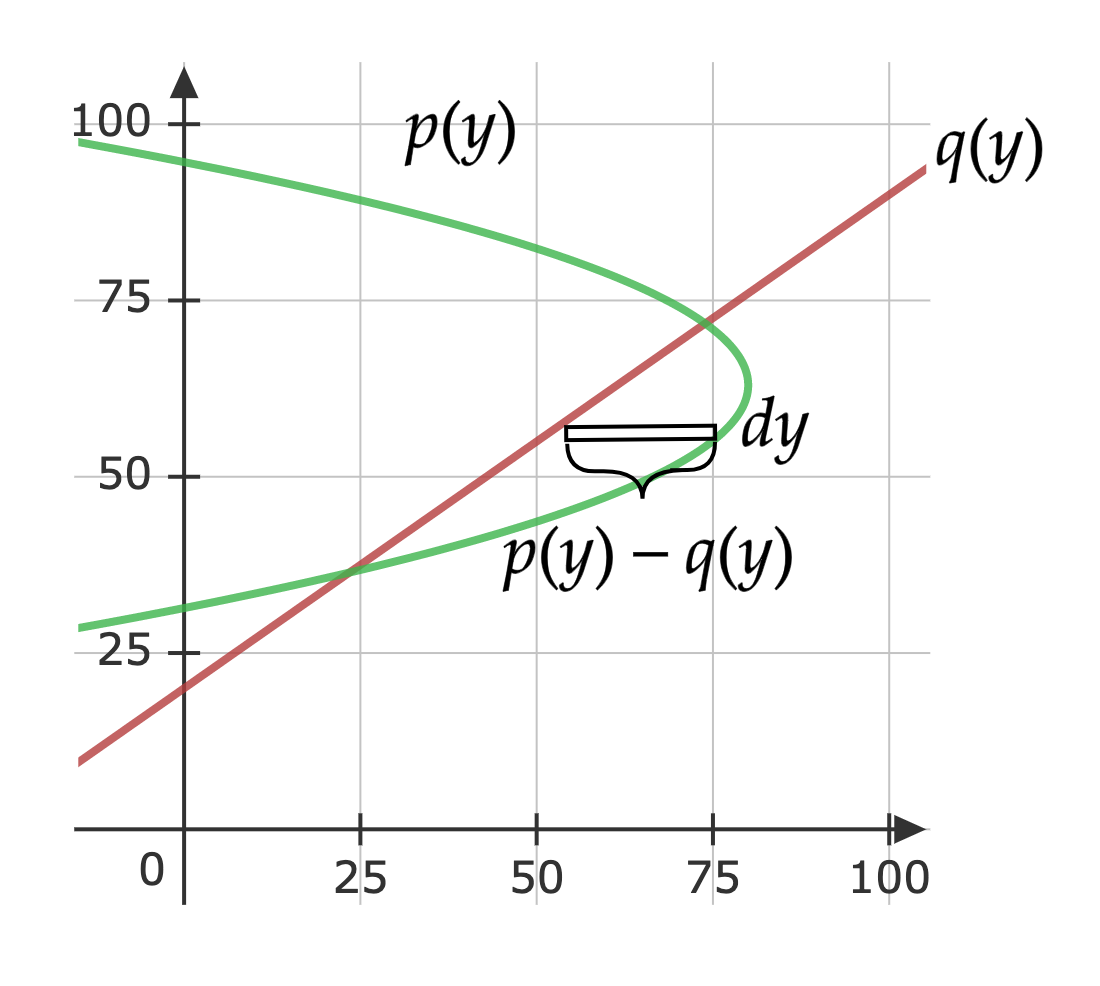
\includegraphics[width=3in]{img/moments_plot2.png}
\end{center}


Keep in mind that $p$ and $q$ are functions in terms of a $y$ variable. If it is difficult to express a function in terms of its $y$ variable, you can still find $\overline{y}$, but you have to be a bit more clever! Here is how:

Remember that when finding $\overline{x}$, we wanted to sum all of the infinitesimal areas along the $x$-axis moment arm and we only cared about the signed distance of the area slice to the $y$-axis. So, analogously, when finding $\overline{y}$, we care that each slice of area that we sum be weighted with the signed distance to the $x$-axis.


We can keep the slices from the $\overline{x}$ sum, we just have to notice that the signed distance on the $y$-axis moment arm (from the $x$-axis) is
$$y=\frac{f(x)+g(x)}{2},$$
the midpoint between the `top' and `bottom' functions. In other words, the midpoint of the area slice is where the mass from the slice is applied to the $y$-axis moment arm. See the figure below for a visual.

\begin{center}
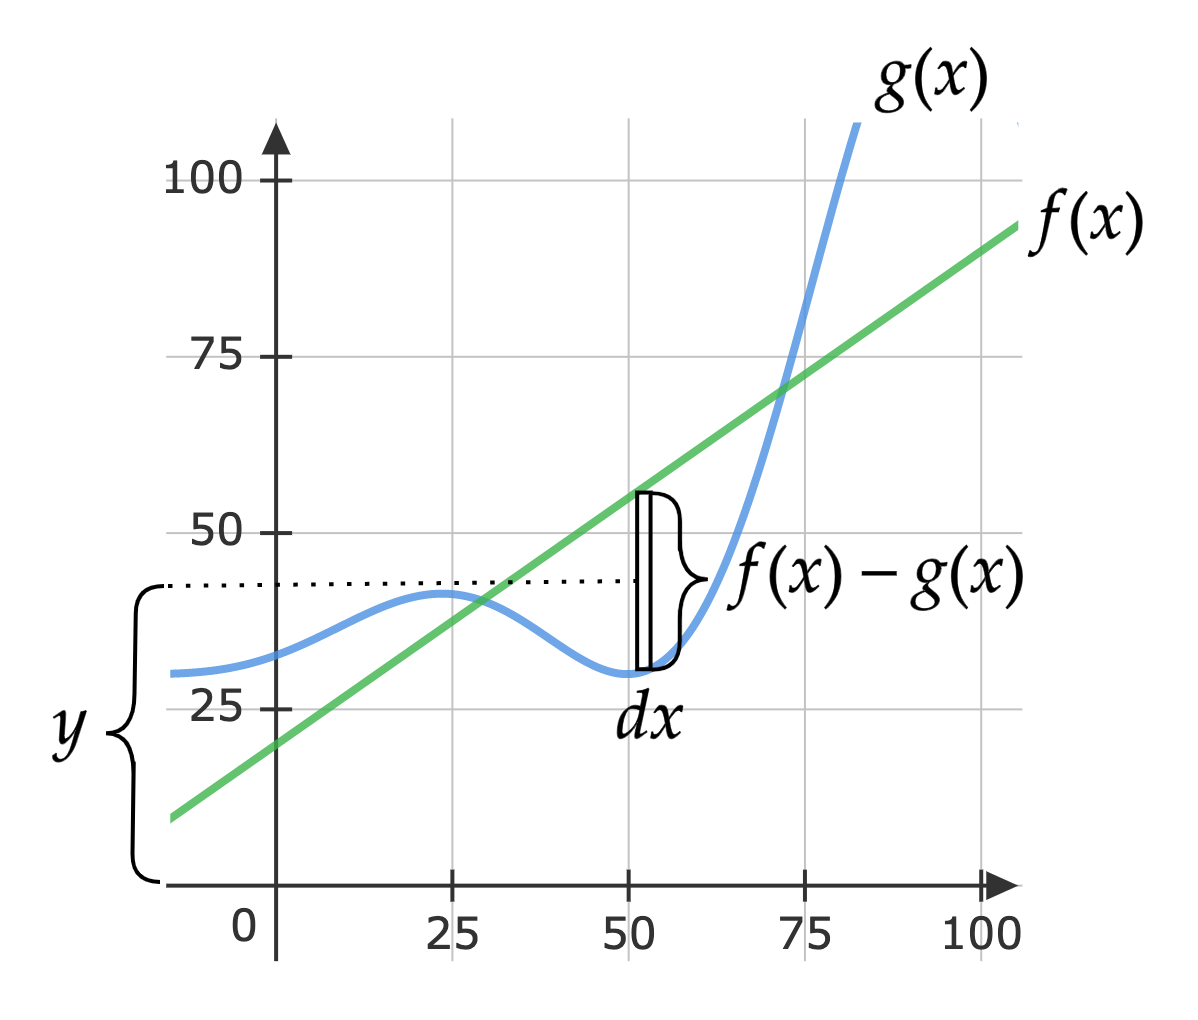
\includegraphics[width=3in]{img/moments_plot3.png}
\end{center}

That means that we can write an integral to find $\overline{y}$ without an integration along the $y$-axis!
$$
\overline{y}=\frac{1}{A}\int_{x=a}^{x=b}\frac{f(x)+g(x)}{2}(f(x)-g(x))\ dx.
$$
If you are interested in finding $\overline{y}$ for the area under a function, then $g(x)=0$, so
$$
\overline{y} = \frac{1}{A}\int_{x=a}^{x=b}\frac{f(x)^2}{2}\ dx.
$$

The point $(\overline{x},\overline{y})$ is called the \textbf{centroid} of a figure in the plane, and is the point on which the figure could balance perfectly along both moment arms.

It is important to know where these formulas come from, as opposed to simply memorizing them. A fundamental part of problem solving is understanding the system you are working in, and being comfortable with adapting methods to fit your needs.

